\section{EndoWrist}\label{sec:Endowrist}

An Endowrist, see \figref{fig:Endo_full} is a surgical tool which can be manipulated in a similar manner as a human wrist with two fingers. Therefore it has four \gls{DOF}, see \figref{fig:Endo_end}. This enables roll, pitch, yaw movement and an open-closing mechanism that acts as the thumb and index finger of a hand.  It is used in surgical procedures such as Laparoscopic surgeries, better known as minimally invasive surgery (MIS), where small incisions in the human body is made during the surgery. Since the incision cuts are small, blood loss during the surgery and the risk of infection is reduced. This has a positive effect on the recovery time for the patient.


\begin{figure}[H]
	\centering
	\begin{subfigure}{.32\textwidth}
		\centering
		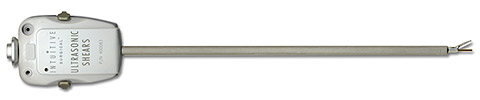
\includegraphics[width=\linewidth]{Endowrist1.jpg}
		\caption{Full view of an EndoWrist\vspace{8.5mm}   }
		\label{fig:Endo_full}
	\end{subfigure}
	\begin{subfigure}{.32\textwidth}
		\centering
		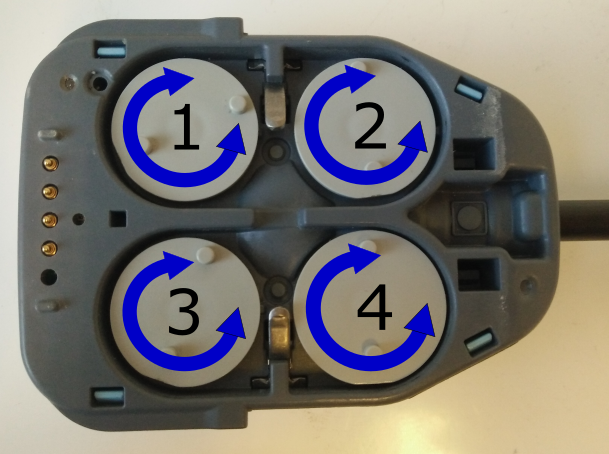
\includegraphics[width=\linewidth]{Endowrist22.png}
		\caption{Actuator plates, which can alternate the end effector position}
		\label{fig:Endo_plates}
	\end{subfigure}
	\begin{subfigure}{.32\textwidth}
		\centering
		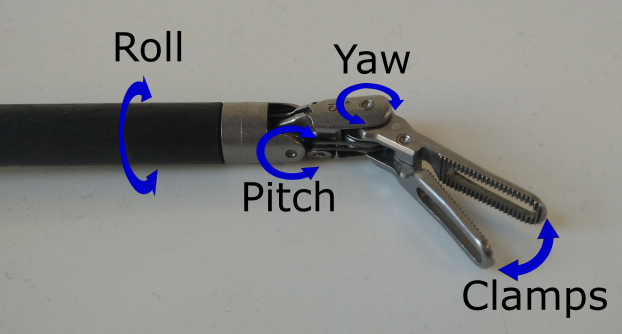
\includegraphics[width=\linewidth,height=3.55cm]{Endowrist31.png}
		\caption{End-effector of the EndoWrist\newline}
		\label{fig:Endo_end}
	\end{subfigure}
\caption{The EndoWrist and how the interaction with it is made}
\label{fig:endowrits_set}
\end{figure}


The end-effector is manipulated by the four wheels seen on \figref{fig:Endo_plates}. Wheel one and three define the movement of the yaw and the closing mechanism for the clamps. Wheel two and four moves the pitch and roll. The EndoWrist is cable driven, which provides the opportunity of making the EndoWrist small. The main drawback of the cable system is that it makes the system nonlinear, since the inherent frition absorbs a significant amount of the input power. Therefore the end-effector's power output is lower than the power input.